% Use only LaTeX2e, calling the article.cls class and 12-point type.

\documentclass[12pt]{article}

% Users of the {thebibliography} environment or BibTeX should use the
% scicite.sty package, downloadable from *Science* at
% www.sciencemag.org/about/authors/prep/TeX_help/ .
% This package should properly format in-text
% reference calls and reference-list numbers.

\usepackage{graphicx}
\usepackage{scicite}
\usepackage{times}
\usepackage{amsthm} 
\usepackage{amsmath} 
\usepackage{amssymb} 
\usepackage{multicol} 
\usepackage{array}
\usepackage{hyperref}

\DeclareMathOperator*{\argmax}{argmax} 
\newtheorem{axiom}{Axiom} 
\newtheorem{theorem}{Theorem}

% The preamble here sets up a lot of new/revised commands and
% environments.  It's annoying, but please do *not* try to strip these
% out into a separate .sty file (which could lead to the loss of some
% information when we convert the file to other formats).  Instead, keep
% them in the preamble of your main LaTeX source file.


% The following parameters seem to provide a reasonable page setup.
\topmargin 0.0cm
\oddsidemargin 0.2cm
\textwidth 16cm 
\textheight 21cm
\footskip 1.0cm


%The next command sets up an environment for the abstract to your paper.
\newenvironment{sciabstract}{%
\begin{quote} \bf}
{\end{quote}}


% If your reference list includes text notes as well as references,
% include the following line; otherwise, comment it out.
\renewcommand\refname{References and Notes}

% The following lines set up an environment for the last note in the
% reference list, which commonly includes acknowledgments of funding,
% help, etc.  It's intended for users of BibTeX or the {thebibliography}
% environment.  Users who are hand-coding their references at the end
% using a list environment such as {enumerate} can simply add another
% item at the end, and it will be numbered automatically.

\newcounter{lastnote}
\newenvironment{scilastnote}{%
\setcounter{lastnote}{\value{enumiv}}%
\addtocounter{lastnote}{+1}%
\begin{list}%
{\arabic{lastnote}.}
{\setlength{\leftmargin}{.22in}}
{\setlength{\labelsep}{.5em}}}
{\end{list}}


% Include your paper's title here
\title{\textbf{Title:} A way around the exploration-exploitation dilemma} 

% Place the author information here.  Please hand-code the contact
% information and notecalls; do *not* use \footnote commands.  Let the
% author contact information appear immediately below the author names
% as shown.  We would also prefer that you don't change the type-size
% settings shown here.
\author
{\textbf{Authors:} Erik J Peterson,$^{1,2\ast}$ Timothy D Verstynen,$^{1,2,3,4}$\\
\\
\normalsize{\textbf{Affiliations:}}\\
\normalsize{$^{1}$Department of Psychology,}\\
\normalsize{$^{2}$Center for the Neural Basis of Cognition,}\\
\normalsize{$^{3}$Carnegie Mellon Neuroscience Institute,}\\
\normalsize{$^{4}$Biomedical Engineering}\\
\normalsize{Carnegie Mellon University, Pittsburgh PA}\\
\\
\normalsize{$^\ast$To whom correspondence should be addressed; E-mail:  Erik.Exists@gmail.com}
}

% Include the date command, but leave its argument blank.
\date{}

%%%%%%%%%%%%%%%%% END OF PREAMBLE %%%%%%%%%%%%%%%%
\begin{document} 
% Double-space the manuscript.
\baselineskip24pt

% Make the title.
\maketitle 

% Place your abstract within the special {sciabstract} environment.
\begin{sciabstract}
  \textbf{Abstract:} The exploration-exploitation dilemma is a fundamental but intractable problem in the learning and decision sciences. In this problem the goal of exploration and exploitation is to maximize reward. Here we challenge this basic form. We conjecture the dilemma can be viewed as a competition between exploiting known rewards or exploring to learn a \emph{world model}, a simplified concept of memory borrowed from computer science. We prove this competition is tractable and can be solved by a simple greedy algorithm. This solution has the properties expected of an optimal solution to original dilemma--finding maximum value with no regret.
\end{sciabstract}

\textbf{One sentence summary:} We prove the intractable exploration-exploitation dilemma can actually be solved by viewing exploitation and exploration as separate goals, that are in competition with each other.

% ----
% \section*{Introduction}
\textbf{Main text:} Let's imagine a bee foraging in a meadow. Our bee has a decision to make. It could go back to the location of a flower it has visited before (exploitation) or go somewhere else (exploration). In a traditional reinforcement learning account when our bee explores it acts to maximize tangible rewards \cite{Sutton2018}, such as finding a plant with more flowers (Figure~\ref{fig:f1}, \textbf{A}). This reinforcement learning account however leads to a mathematically intractable dilemma over whether it is optimal to explore or exploit a any given moment \cite{Thrun1992a,Dayan1996,Findling2018,Gershman2018b}. 

Resource gathering is not the only reason animals explore. Many animals, like our bee, learn simplified models of the world to make decisions and plan actions \cite{Ahilan2019,Poucet1993}. Borrowing from the field of artificial intelligence we refer to these as world models \cite{Schmidhuber2019,Sutton2018,Schmidhuber1991}. When learning a world model, information about the environment is intrinsically valuable and is why animals are intrinsically curious \cite{Mehlhorn2015,Gupta2006,Berger-Tal2014,Gottlieb2018,Schwartenbeck2019,Pathak2017} and prone to explore even when no rewards are present or expected \cite{Hughes1997}. In some cases information seeking is known to happen even if it explicitly leads to a loss of reward \cite{Wang2019}. 

Here we conjecture that the only kind of exploratory behavior an animal needs to do is that which builds its world model. With this conjecture we can propose an alternative to the classic dilemma, breaking exploration and exploitation into independent objectives that compete to either exploit known rewards or explore to learn a world model (Figure~\ref{fig:f1}\textbf{B}). We prove this alternative has a tractable and optimal solution. Optimal here means maximising rewards while minimizing regrets.

\begin{figure}
	[tbhp] \centering 
	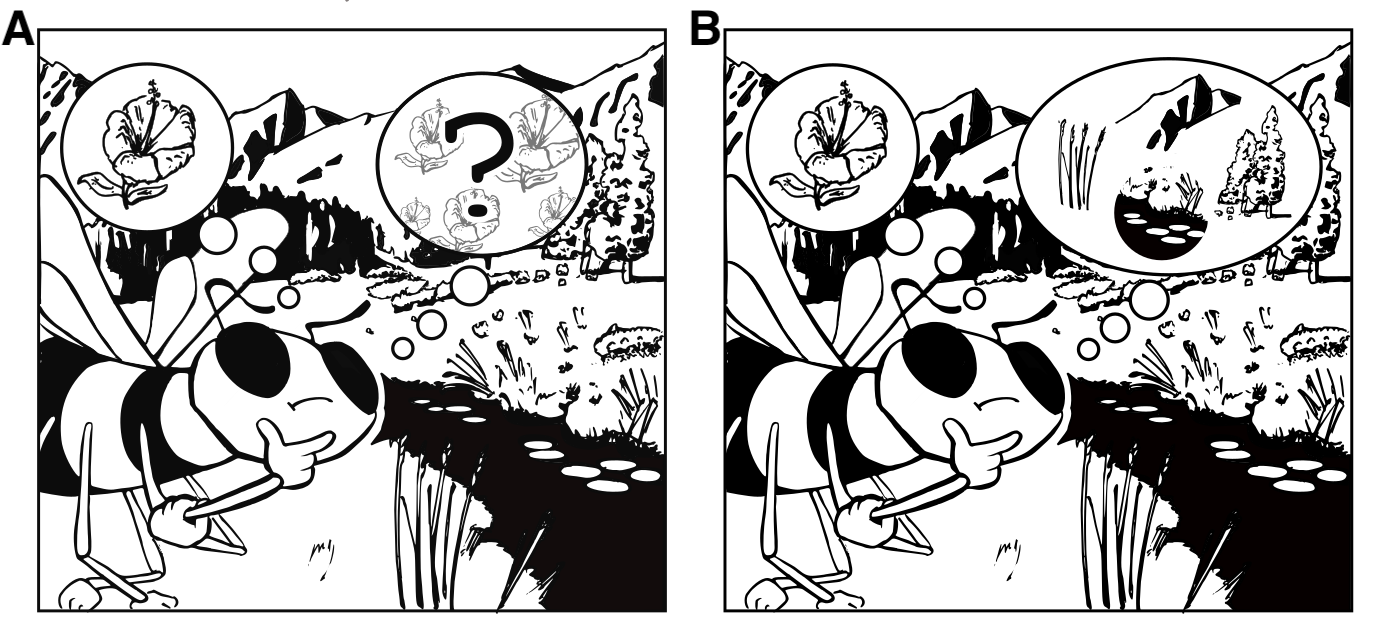
\includegraphics[width=.7\linewidth]{figures/fig1.png} 
	\caption{\label{fig:f1} Two views of exploration and exploitation. \textbf{A}. The classic dilemma is depicted as two options for reward maximization: exploit an action with a known reward likelihood (e.g., return to the previous plant) or stochastically explore other actions on the chance they return better outcomes (e.g., find a plant with more flowers). \textbf{B.} Here we offer an alternative view of the dilemma, with two different competitive goals: maximize rewards (e.g., keep returning to known flower locations) \texti{or} build a model of the world by learning new information (e.g., layout of the environment). Notice how exploration here is based not on finding rewards per se (e.g., flowers), but on learning in general. \textit{Artist credit}: Richard Grant.}
\end{figure}

Our contribution is threefold. We offer five axioms that serve as a general basis to estimate the value of any learned observation, given a memory. This prospective leads to a surprising result. Information theory can be formally disconnected from information value, producing a new universal theory. Next we prove that the computer science method of dynamic programming \cite{Bellmann1954,Sutton2018} provides an optimal way to maximize this kind of information value. Finally, we describe a simple greedy scheduling algorithm that can maximize both information value and reward.


% \section*{Results}
% \subsection*{A definition of information value}
Rewards and information are fundamentally distinct concepts. Rewards are a conserved resource. Information is not. For example if a rat shares potato chip with a cage-mate, she must necessarily split the chip up leaving less food for herself. Whereas if student shares the latest result from a scientific paper with a lab-mate, they do not necessarily forget a portion of that result.

To formally separate the value of information from the value of reward we look to the field of information theory \cite{Shannon1948}. Rather than focus on the statistical problem of transmitting symbols, as was Shannon’s goal, we focus on remembering symbols, in order to produce a learning and memory view of information value. 

World models are memories that range from simple novelty signals \cite{Kakade2002}, to location or state counts \cite{Bellemare2016,Dayan1993}, state and action prediction \cite{Schmidhuber1991,Pathak2017,Friston2016}, flow \cite{Yang2019}, learning progress \cite{Lopes2012}, classic working or episodic memories \cite{Miller1956,Tulving2002}, Bayesian and hierarchical Bayesian models \cite{Park2017,Itti2009,Friston2016,Tenenbaum2006}, latent spaces \cite{Kingma2013} and recurrent neural networks \cite{Ganguli2008,Ha2018,Schmidhuber2015a,Mante2013}. In all of these examples, the value of any observation made by an agent who is learning a world model depends entirely on what the agent learns by making that observation.

We do not prefer any one kind of world model to any other. So we adopt a broad definition of memory, which overlaps with nearly any world model. We assume that time $t$ is continuous quantity, and denote increases in time using the differential quantity $dt$. We generally then express changes in $M$ (our memory, defined below) as a differential equation (e.g., $\frac{dM}{dt}$), although for non-differential memories difference equations can be used (e.g., $\frac{\Delta M}{\Delta t}$). 

Observations about the environment $s$ are real numbers sampled from a finite state space $s \in S$, whose size is $N$ (denoted $S^N$). Actions are also real numbers $a$ drawn from a finite space $A^K$. Rewards $R_t$, when they appear, are generally binary and always provided by the external environment. 

Preliminaries aside, we can formally define a memory $M$ as a finite set of real numbers, whose maximum size is also $N$ ($M^N$). We say that learning of $s$ at time $t$ by $M$ happens by an invertible encoder function $f$, $M_{t+dt} = f(M_{t}, s_{t})$ and $M_{t} = f^{-1}(M_{t+dt}, s_{t})$. (Invertibility here is equivalent to saying that any observations which be stored can be forgotten). Memories $\hat s_t$ about $s_t$ are recalled by a decoder function $g$, such that $\hat s_t = g(M_t, s_t)$. 

The details of $f$ and $g$ define what kind of world model $M$ is. To make this more concrete, let's consider some examples. If $f$ simply adds states to the memory and $g$ tests whether $s_t$ is in $M$, then $M$ models novelty \cite{Kakade2002}. If $f$ counts states and $g$ returns those counts, then $M$ is a count-based heuristic \cite{Bellemare2016,Dayan1993}. If $f$ follows Bayes rule and $g$ decodes the probability of $s_t$, then we have recovered a classic frequently used information theory account of information value \cite{Itti2009,Friston2016,Tenenbaum2006}. In this account the decoded state probabilities could be the current state, or for future states or actions \cite{Schmidhuber1991,Pathak2017,Friston2016}. Or if $M$ is much smaller than the size of the space $S^N$, then $f$ could learn a latent or compressed representation \cite{Kingma2013,Schmidhuber2008,Levi-Aharoni2019,Ganguli2010,Ha2018,Schmidhuber2015a,Mante2013,Park2017}, with $g$ decoding a reconstruction of current ($\hat s_t$) or future states ($\hat s_{t+dt}$).

We define a real valued distance $E$ to measure how $M$ changes with both time and observations. Different $f$ and $g$ pairs will naturally need different ways to exactly express this distance. For example, a novelty model \cite{Kakade2002} would produce binary values, as would a count model \cite{Bellemare2016,Dayan1993}. A latent memory \cite{Schmidhuber1991,Pathak2017} might use its own error gradient. A probabilistic memory \cite{Park2017,Friston2016} would likely use the KL divergence. All that matters is the chosen distance meet our five axioms. 

\begin{axiom}
	[Axiom of Memory] $E(s_t)$ depends \emph{only} on how the memory $M$ changes when making an observation $s_t$. 
\label{ax:1} \end{axiom}
\begin{axiom}
	[Axiom of Novelty] An observation $s_t$ that doesn't change the memory $M$ has no value. $E(s_t) = 0$ if and only if $\frac{dM}{dt} = 0$. 
\label{ax:2} \end{axiom}
\begin{axiom}
	[Axiom of Scholarship] All learning in $M$ about $s_t$ is valuable. $E(s_t) \geq 0$; $\frac{dM}{dt} \geq 0$. 
\label{ax:3} \end{axiom}
\begin{axiom}
    [Axiom of Specificity] If the total change in memory $M$ due to observation $s_t$ is held constant ($\frac{dM}{dt} = h$), the more compact (Eq.~\ref{eq:compactcude}) the change in memory the more valuable the observation. 
\label{ax:4} \end{axiom}
\noindent Axiom~\ref{ax:4} adds two critical and intertwined properties. It ensures that if all else is held equal, more specific observations are more valuable that less specific observations \cite{Berlyne1950,Kidd2015}. It also ensures that an observation that leads to a simplifying or parsimonious insight (is equivalent to a compression of the memory, \cite{Schmidhuber2008}) is more valuable than one that changes memory the same total amount but does not lead to compression.
\begin{axiom}
	[Axiom of Equilibrium] An observation $s_t$ must be learnable by $M$. $\frac{d^2M}{dt^2} \leq 0$. 
\label{ax:5} \end{axiom}
\noindent Technically speaking by learnable we mean learnable using the probably approximately correct (PAC) framework \cite{Valiant1984}, a common tool of computer science used to formalize learning and inference. Any observation that cannot be learned, for whatever the reason, is not valuable because it cannot change behavior.

Having written down a positive definition, for clarity we'll also state what our theory is not. Information value is not based on the intrinsic complexity of an observation (that is, its entropy) \cite{Haarnoja2018}, nor on its similarity to the environment (its mutual information; \cite{Kolchinsky2018}), nor on its novelty or surprise \cite{Itti2009,Friston2016,Dayan1996}. 

Stimulus complexity and surprise have tremendous potential to drive learning, of course. In cases like Bayesian rule there is even a fixed relationship between learning and surprise \cite{Itti2009,Friston2016,MacKay2003}. However, this does not hold for all learning rules. Complexity and surprise which can't be learned is not valuable; if it can't be learned it can't shape future actions. 

% \subsection*{Exploration as a dynamic programming problem}
Dynamic programming is a popular optimization approach because it can guarantee total value is maximized by a simple, deterministic, and greedy algorithm. In Theorem~\ref{theorem:opt_sub} (see Mathematical Appendix) we prove our definition of memory has one critical property, optimal substructure, that is needed for a greedy dynamic programming solution \cite{Bellmann1954,Roughgarden2019}. The other two needed properties, $E \ge 0$ and the Markov property \cite{Bellmann1954,Roughgarden2019}, are fulfilled by the Axioms 3 and 1 respectively. 

To write down dynamic programming (or Bellman) solution for $E$ we must introduce a little more notation. We let $\pi$ denote the action policy, a function that takes a state $s$ and returns an action $a$. We let $\delta$ be a transition function that takes a state-action pair $(s_{t},a_t)$ and returns a new state, $s_{t+dt}$. For notational simplicity we also redefine $E$ as $F(M_{t}, a_t)$, and call this the \textit{payoff function} \cite{Bellmann1954}.
 
\begin{equation}
	\begin{split}\label{eq:payout} 
		F(M_{t}, a_t) = E(s)\\
		\text{subject to the constraints} \\
		a_{t} = \pi(s_t) \\
		s_{t+dt} = \delta(s_{t}, a_t),\\
		M_{t+dt} = f(M_{t}, s_{t}) 
	\end{split}
\end{equation}

\noindent The value function for $F$ is,

\begin{equation}\label{eq:V_E} 
	\begin{split}
		V_{\pi_E}(M_0) = \Big [ \max_{a \in A} \sum_{t=0}^{\infty} F(M_t, a_t) \ \Big | \ M,\ S,\ A \Big ]. 
	\end{split}
\end{equation}

\noindent And the recursive Bellman solution to learn this value function is,

\begin{equation}\label{eq:bellman_iter} 
	V^*_{\pi_E}(M_{t}) = F(M_{t}, a_{t}) + \max_{a \in A} \Big [ F(M_{t+dt}, a_t) \Big ].
\end{equation}

For the full derivation see the \textit{Mathematical Appendix}. Eq.~\ref{eq:bellman_iter} implies that the optimal action policy $\pi^*_E$ for $E$ (and $F$) is a simple greedy policy. This greedy policy ensures that exploration of any finite space $S$ is exhaustive (Theorems~\ref{theorem:Z} and~\ref{theorem:convergence} in Mathematical Appendix).

Axiom~\ref{ax:5} requires that learning in $M$ converge. Axiom~\ref{ax:4} requires information value increases with surprise, re-scaled by specificity. When combined with a greedy action policy like $\pi^*_E$, these axioms naturally lead to active learning \cite{Shyam2018,Pathak2019,Schwartenbeck2019} and to adversarial curiosity \cite{Schmidhuber2019a}.

% \subsection*{Scheduling a way around the dilemma} 
Remember that the goal of reinforcement learning is to maximize reward, an objective approximated by the value function $V_R(s)$ and an action policy $\pi_R$. 

\begin{equation}\label{eq:V_R} 
	V^{\pi_R}_R(s) = \mathbb{E} \Big [ \sum_{k=0}^{\infty} R_{t+k+1} \big | s = s_t \Big ] 
\end{equation}

To find an algorithm that maximizes both information and reward value we imagine the policies for exploration and exploitation acting as two possible ``jobs'' competing to control behavior. For exploration and exploitation we know (by definition) each of these jobs produces non-negative values which an optimal job scheduler could use: $E$ for information or $R$ for reward/reinforcement learning. Finding an optimal scheduler turns out to require we further simplify our assumptions. 

We assume we are in a typical reinforcement learning setting, which is where the dilemma finds its simplest expression anyway. In this setting rewards are either present or absent (0, 1). Each action takes a constant amount of time and has no energetic cost. And each policy can only take one action at a time. 

Most scheduling problems also assume that the value of a job is fixed, while in our problem information value changes as the memory learns and we expect that rewards are stochastic. However, in a general setting where one has no prior information about the environment the best predictor of the next future value is very often the last value \cite{Hocker2019,Roughgarden2019}. We assume this precept holds in all of our analysis.

The optimal solution to a scheduling problem with non-negative values and fixed run times is a deterministic greedy algorithm \cite{Roughgarden2019}. We restate this solution as a set of inequalities where $R_t$ and $E_t$ represent the value of reward and information at the last time-point.

\begin{equation}
\label{eq:pipi} 
	\begin{split}
		\pi_{\pi}(s_t) = 
		\begin{cases}
			\pi^*_E(s_t) & : E_t - \eta > R_t \\
			\pi_R(s_t) & : E_t - \eta \le R_t \\
		\end{cases}
		\\
		\text{subject to the constraints}\\
		p(\mathbb E[R]) < 1 \\
		E - \eta \geq 0
	\end{split}
\end{equation}

To ensure that the default policy is reward maximization, Eq.~\ref{eq:pipi} breaks ties between $R_t$ and $E_t$ in favor of $\pi_R$. In stochastic environments, $M$ can show small continual fluctuations. To allow Eq.~\ref{eq:pipi} to achieve a stable solution we introduce $\eta$, a boredom threshold for exploration. Larger values of $\eta$ devalue exploration.

Reframing the exploration-exploitation dilemma as a scheduling problem comes at the cost of increasing overall computational complexity \cite{Valiant1984}. The worst case run time for $\pi_{\pi}$ is linear and additive in its policies. That is, if in isolation it takes $T_E$ steps to earn $E_{T} = \sum_{T_E} E$, and $T_R$ steps to earn $r_{T} = \sum_{T_R} R$, then the worst case training time for $\pi_{\pi}$ is $T_E + T_R$. This is only true  if neither policy can learn from the other's actions. There is, however, no reason that each policy cannot observe the transitions $(s_t, a_t, R, s_{t+dt})$ caused by the other. If this is allowed, worst case training time improves to $\max(T_E, T_R)$.

% \subsection*{Exploration without regret} 
Suboptimal exploration strategies will lead to a loss of potential rewards by wasting time on actions that have a lower expected value. Regret $G$ measures the value loss caused by such exploration. $G = \hat V - V_a$, where $\hat V$ represents the maximum value and $V_a$ represents the value found by taking an exploratory action rather than an exploitative one \cite{Sutton2018}. 

Optimal strategies for a solution to the exploration-exploitation dilemma should maximize total value with zero total regret. 

\begin{figure}
	[tbhp] \centering 
	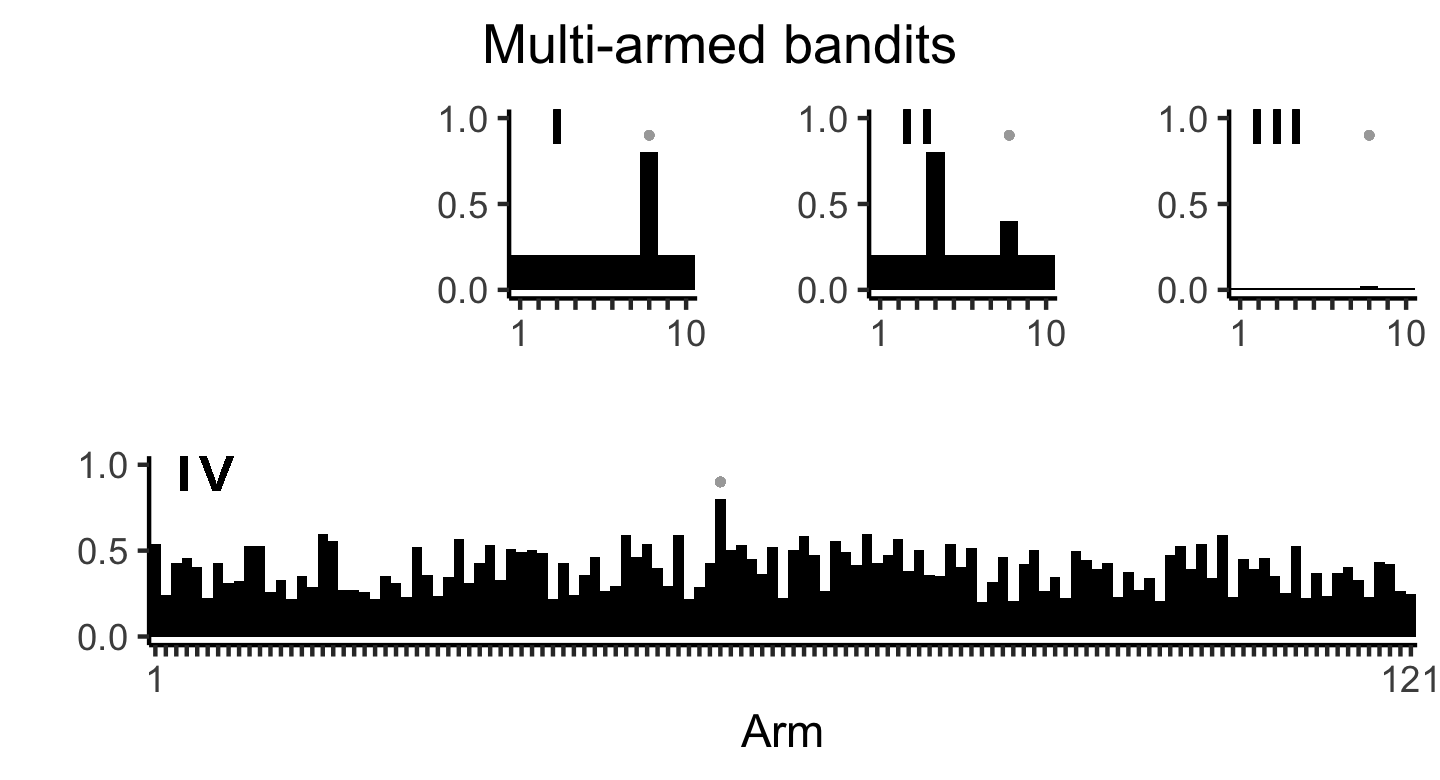
\includegraphics[width=.6\linewidth]{figures/fig2.png} 
	\caption{ \label{fig:f2} Bandits. Reward probabilities for each arm in bandit tasks I-IV. Grey dots highlight the optimal (i.e., highest reward probability) arm. See main text for a complete description.} 
\end{figure}

\begin{figure}
	[tbhp] \centering 
	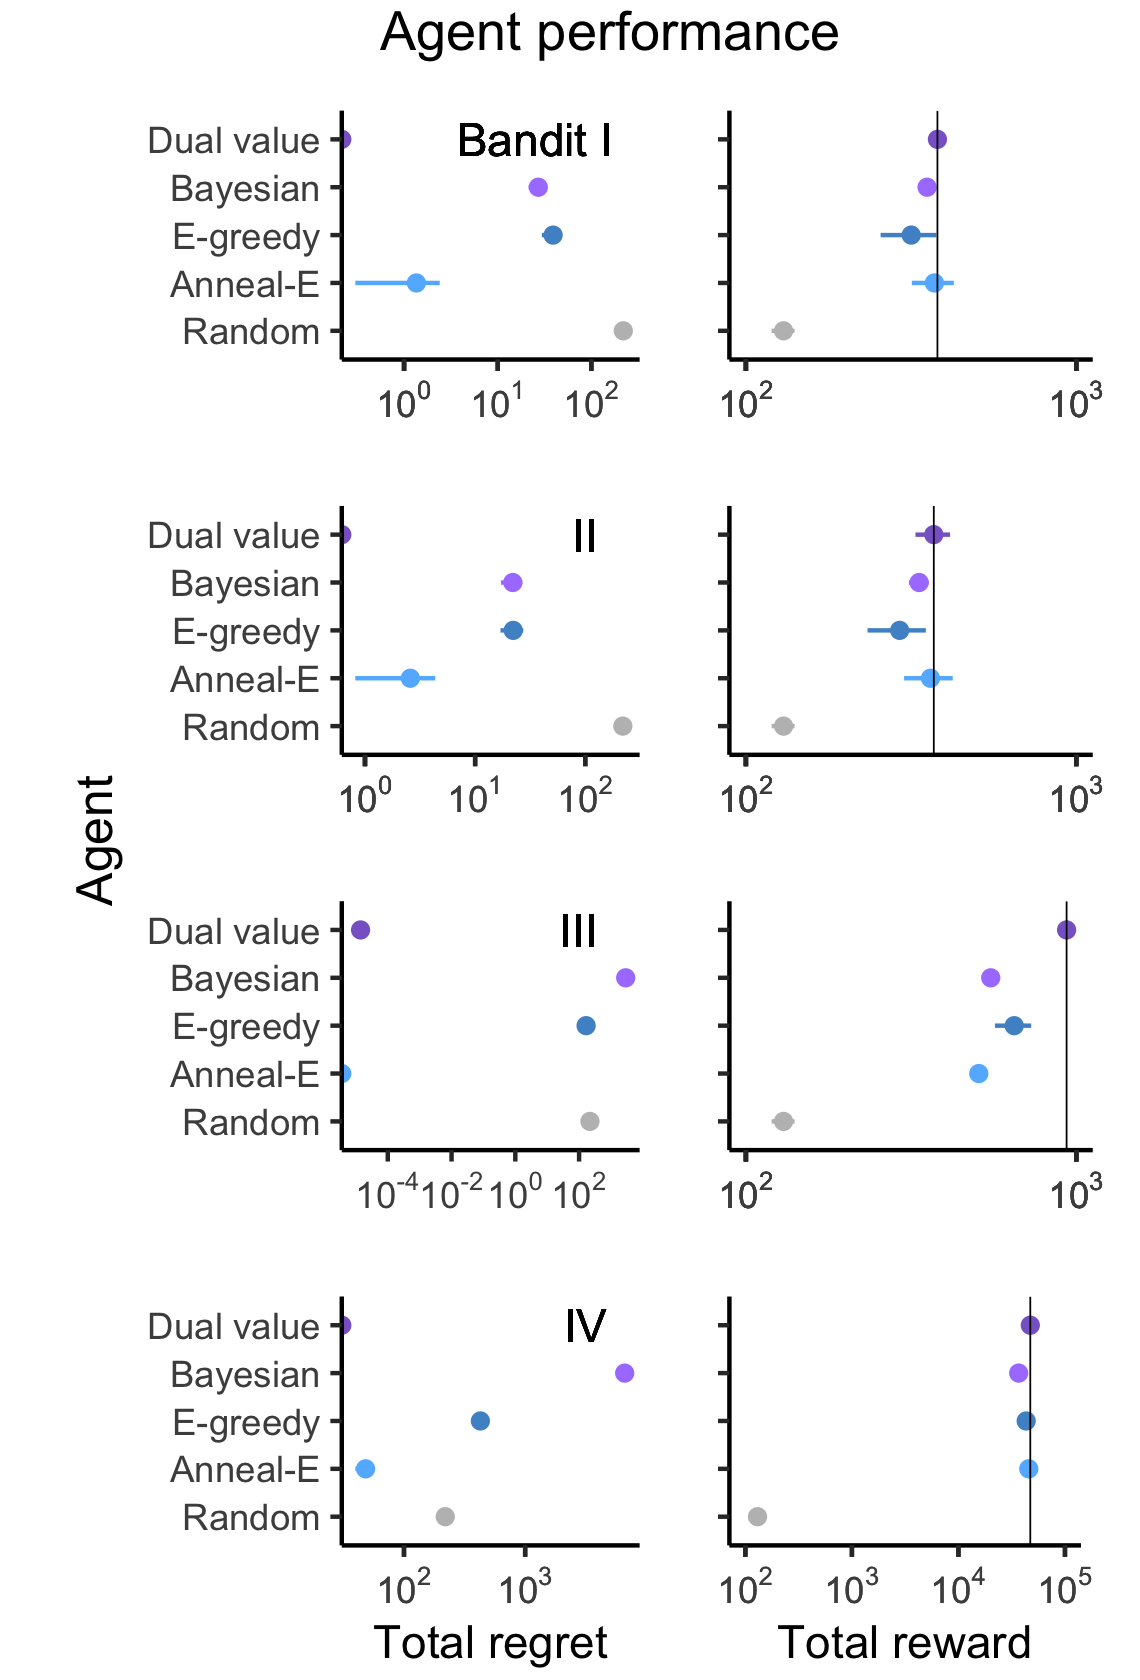
\includegraphics[width=.45\linewidth]{figures/fig3.png} 
	\caption{ \label{fig:f3} Regret and total accumulated reward across models and bandit task. Median total regret (left column) and median total reward (right column) for simulations of each model type ($N=100$ experiments per model). See main text and Table~\ref{tab:agents} for description of each model. Error bars in all plots represent median absolute deviation.} 
\end{figure}

To evaluate dual value learning (Eq.~\ref{eq:pipi}) we compared total reward and regret across a range of both simple, and challenging multi-armed bandit tasks. Despite its apparent simplicity, the essential aspects of the exploration-exploitation dilemma exist in the multi-armed task \cite{Sutton2018}. Here the problem to be learned is the distribution of reward probabilities across arms (Figure ~\ref{fig:f2}).  To estimate the value of any observation $s_t$, we compare sequential changes in this probabilistic memory, $M_{t+dt}$ and $M_t$ using the KL divergence (i.e. relative entropy; Figure \ref{fig:supf1}\textbf{A}-\textbf{B}). The KL divergence is a standard way to measure the distance between two distributions \cite{MacKay2003} and is, by design, consistent with the axioms (see the Supplementary Materials for a more thorough discussion). 

We start with a simple experiment with a single high value arm. The rest of the arms have a uniform reward probability (Bandit \textbf{I}). This represents a trivial problem. Next we tried a basic exploration test (Bandit \textbf{II}), with one winning arm and one distractor arm whose value is close to but less than the optimal choice. We then move on to a more difficult sparse exploration problem (Bandit \textbf{III}), where the world has a single winning arm, but the overall probability of receiving any reward is very low ($p(R) = 0.02$ for the winning arm, $p(R) = 0.01$ for all others). Sparse reward problems are notoriously difficult to solve, and are a common feature of both the real world and artificial environments like Go, chess, and class Atari video games \cite{Mniha,Silver2016b,Silver2018}. Finally, we tested a complex, large world exploration problem (Bandit (\textbf{IV}) with 121 arms, and a complex, randomly generated reward structure. Bandits of this type and size are near the limit of human performance \cite{Wu2018}. 

We compared the reward and regret performance of 6 artificial agents. All agents used the same temporal difference learning algorithm (TD(0), \cite{Sutton2018}). The only difference between the agents was their exploration mechanism (Table~\ref{tab:agents}; for a complete description see the \textit{Supplementary materials}). 

\newcolumntype{L}{>{\arraybackslash}m{6cm}} 
\begin{table}[] 
    \centering 
	\caption{Artificial agents.} \label{tab:agents} 
	\begin{tabular}
		{|l|L|} \hline \textbf{Agent} & \textbf{Exploration mechanism} \\
		\hline Dual value & Our algorithm (Eq~\ref{eq:pipi}). \\
		\hline E-greedy & With probability $1-\epsilon$ follow a greedy policy. With probability $\epsilon$ follow a random policy. \\
		\hline Annealed e-greedy & Identical to E-greedy, but $\epsilon$ is decayed at fixed rate. \\
		\hline Bayesian reward & Use the KL divergence as a weighted intrinsic reward, sampling actions by a soft-max policy. $\sum_T R_t + \beta E_t$ \\
		\hline Random & Action are selected with a random policy (no learning) \\
		\hline 
	\end{tabular}
\end{table}

All of the classic and state-of-the-art algorithms performed well at the different tasks in terms of accumulation of rewards (right column, Figure \ref{fig:f3}). The one exception to this being the sparse low reward probability condition (Bandit \textbf{III}), where the dual value algorithm consistently returned more rewards than the other models. In contrast, most of the traditional models still had substantial amounts of regret in most of the tasks, with the exception of the annealed variant of the e-greedy algorithm during the sparse, low reward probability task (left column, Figure~\ref{fig:f3}). In contrast, the dual value learning algorithm consistently was able to maximize total reward with zero or near zero (Bandit \textbf{III}) regret, as would be expected by an optimal exploration policy.

% \subsection*{Discussion}
% TODO - real short summary.
Since Schultz \textit{et al}’s \cite{Schultz1998} report showing dopamine neurons behave quantitatively like a reward prediction error signal, reinforcement learning has been central to the study of learning \cite{Neftci2019}, as well as important to our conception of numerous neurological and psychiatric disorders, including autism \cite{Sinha2014} and schizophrenia \cite{Maia2017}. Reinforcement learning is also undergoing a renaissance in artificial intelligence research, achieving superhuman performance on Atari video games \cite{Mnih2015}, chess \cite{Silver2018}, and Go \cite{Silver2016}. However, despite this progress all of reinforcement learning shares a common dilemma without a formal solution. Here we suggest a related problem, a simple competition, that both has a solution itself and has the properties of an ideal solution to the dilemma itself; maximum value with zero regret. 

Naturalistic accounts of exploratory behavior at present rely on probabilistic models \cite{Calhoun2014,Song2019a,Gershman2018b,Schulz2018a}. Our theory predicts it should be possible to guide exploration in real-time using, for example, optogenetic methods in neuroscience, or well timed stimulus manipulations in economics or other behavioral sciences.

Our theory also has may lead to new progress in artificial intelligence research, which is limited by three factors: data efficiency, exploration efficiency, and transfer learning \cite{Sutton2018,Ha2018,Kulkarni2016a} (see the \textit{Supplementary Discussion} for a complete explanation of these points).

% \subsection*{Everyday life}
Our most important contribution is perhaps a better worldview on a hard and common problem.

\textbf{Q}: Should we eat at our favorite, or try the new restaurant down the street? What if it's bad?
\textbf{A}: I'm not sure\ldots

Even in a mundane setting like this question, and its dilemma, the potential loss from exploration is daunting and uncertain to think about. Well beyond the mundane, variations on this problem are universal appearing in psychology, neuroscience, biology, data science, artificial intelligence, game theory, economics, demography, and political science. Here we suggest an universal alternative.

The uncertainty of the unknown can always be recast as an opportunity to learn. But rather than being a trick of psychology, we prove this view is (in the narrow sense of our formalism anyway) mathematically optimal.

\textbf{Q}: Would I rather have this reward, or learn something new? 
\textbf{A}: Which do I value more right now? Pick the biggest.

\bibliographystyle{Science}
\bibliography{library}

\textbf{Acknowledgments:} EJP and TV wish to thank Jack Burgess, Matt Clapp, Kyle Donovank, Richard Gao, Roberta Klatzky, Jayanth Koushik, Alp Muyesser, Jonathan Rubin, and Rachel Storer for their comments on earlier drafts. EJP also wishes to thank Richard Grant for his illustration work in Figure 1. \textbf{Funding:}The research was sponsored by the Air Force Research Laboratory (AFRL/AFOSR) award FA9550-18-1-0251. The views and conclusions contained in this document are those of the authors and should not be interpreted as representing the official policies, either expressed or implied, of the Army Research Laboratory or the U.S. government. TV was supported by the Pennsylvania Department of Health Formula Award SAP4100062201, and National Science Foundation CAREER Award 1351748. \textbf{Authors contributions:} EJP conceived of the idea, designed the research and developed the proofs, and wrote the manuscript. TV designed the research and wrote the manuscript. \textbf{Data and materials availability:} All code and data is available at \url{https://github.com/CoAxLab/infomercial}.

%%%%%%%%%%%%%%%%%%%%%%%%%%%%%%%%%%%%%%%%%%%%%%%%%%%%%%%%%%%%%%%%%%%%%%%%%%%%
% --------------------------------------------------------------------------
%%%%%%%%%%%%%%%%%%%%%%%%%%%%%%%%%%%%%%%%%%%%%%%%%%%%%%%%%%%%%%%%%%%%%%%%%%%%
\section*{Mathematical Appendix.}
\newcommand{\beginsupplement}{%
        \setcounter{table}{0}
        \renewcommand{\thetable}{S\arabic{table}}%
        \setcounter{figure}{0}
        \renewcommand{\thefigure}{S\arabic{figure}}%
     }
\beginsupplement
\setcounter{theorem}{0}

% --------------------------------------------------------------------------
\subsection*{Optimal substructure in memory}
To find an optimal value solution for $\hat E$ using the Bellman equation we must prove our memory $\mathbf{M}$ has optimal substructure. This is because the normal route, which assumes the problem rests in a Markov Space, is closed to us. By optimal substructure we mean that the process of learning in $\mathbf{M}$, and therefore maximization of $\hat E$ can be partitioned into a collection, or series of memories, each of which is itself an max value solution.

This opaque term of optimal substructure can be intuitivily understood by looking in turn at another theoretical construct, Markov spaces. 

In Markov spaces there are a set of states $(S_0, S_1, \ldots)$, where the transition to the next $S_t$ depends only on the previous state $S_{t-1}$. This limit means that if we were to optimize over these states, as in reinforcement learning, we know that we can treat each transition as its own ``subproblem'', and ignore the history's $(S_0, S_1, \ldots)$ effect on value, and therefore the overall situation has ``optimal substructure''.

The problem for our defintion of information value is it relies on memory which is necessarily composed of many past observations, in many orders, and so it cannot be a Markov space. So if we wish to use the Bellman equation, we need to find another way to establish optimal substructure. This is the focus of Theorem~\ref{theorem:opt_sub}. In this theorem we implicitly assume that $\mathbf{X} = \mathbf{S}$, $\mathbf{A}$, $\mathbf{M}$, $f$, and $\Lambda$ are given, and that $\Lambda$ is deterministic, 

\begin{theorem}[Optimal substructure] \label{theorem:opt_sub} 
   If $V^*_{\pi_{\hat E}}$ is the optimal information value given by policy $\pi_{\hat E}$, a memory $\mathbf{M}_t$ has optimal substructure if the last observation $X$ can be removed from $\mathbf{M}$, by $\mathbf{M-1}_{t} = f^{-1}(\mathbf{X}, \mathbf{M}_t)$ such that the resulting value $V^*_{t-1} = V^*_{t} - E_{t}$ is also optimal. 
\end{theorem}
\begin{proof}
	Given a known optimal value $V^*$ given by $\pi_{\hat E}$ we assume for the sake of contradiction there also exists an alternative policy $\hat \pi_{\hat E} \neq \pi_{\hat E}$ that gives a memory $\hat{\mathbf{M}}_{t-1} \neq \mathbf{M}_{t-1}$ and for which $\hat V^*_{t-1} > V^*_{t-1}$. 
	
	To recover the known optimal memory $\mathbf{M}_t$ we lift $\hat{\mathbf{M}}_{t-1}$ to $\mathbf{M}_t = f(\hat{\mathbf{M}}_{t-1}, \mathbf{X}_t)$. This implies $\hat V^* > V^*$ which in turn contradicts the purported original optimality of $V^*$ and therefore $\hat \pi_{\hat E}$.
\end{proof}

This proof requires two things. First, we need to a mechanism of forgetting, of a very particular kind. We assume that the last learning step $f(\mathbf{X}, \mathbf{M}) \rightarrow \mathbf{M}'$ can be undone by a new vector valued function $f^{-1}$, such that $f(\mathbf{X}, \mathbf{M'}) \rightarrow \mathbf{M}$. In other words we must assume what was last remembered, can always be exactly forgotten. Second, we assume the environmental dynamics, given by the transition function $\Lambda$, are deterministic. 

Determinism is consistent with the natural world which does evolve in a deterministic way, at the scale of animal behavoir that we concerned with at least. This assumption is however at odds with much of reinforcement learning theory \cite{Sutton2018} and past experimental work. For example, \cite{Gershman2018}. Both tend to study stochastic environments. We addressed this discrepancy in the main text, using numerical simulations.


% ------------------------------------------------------------------------
\subsection*{Bellman optimal information collection}
We aim to find a series of actions $(\mathbf{A}_1, \mathbf{A}_2, ..\mathbf{A}_T)$, drawn from a set $\mathbb{A}$, that maximize each payout $(\hat E_0, \hat E_1, \ldots, \hat E_{T})$ so the total payout received is as large as possible. If there is a policy $\mathbf{A} = \pi(\mathbf{X})$ to take actions, based on a series of observations $(X_0, X_1, ..X_{T}),$, given by $\Lambda$, then an optimal policy $\pi^*$ will always find the maximum total value $V^* = \argmax_{\mathbf{A} \in \mathbb{A}} \sum_T \hat E_t $. In the form above one would need to reconsider the entire sequence of actions for any one change to that sequence, leading to a combinatorial explosion. Bellman's insight was a way to make this last problem simpler by breaking it down into a small set of subproblems that we can solve in a tractable way without an explosion in complexity. This is his principle of optimality, which reads:

\begin{quote}
    An optimal policy has the property that whatever the initial state and initial decision are, the remaining decisions must constitute an optimal policy with regard to the state resulting from the first decision. \cite{Bellmann1954}
\end{quote}

Mathematically Bellman's principle allows us to translate the full problem, $V^* = \argmax_{\pi} \sum_T \hat E_1, \hat E_2, ..., \hat E_{T}$ to a recursive one. Having already proven the optimal substructure of $\mathbf{M}$, and given an arbitrary starting value $E_0$, the Bellman solution to curiosity optimization of $\hat E$ is therefore given by,

\begin{equation} 
	\label{eq:bellman_iter_E_app}
	V^*_{\hat E}(\mathbf{S}) = \argmax_{\mathbf{A} \in \mathbb{A}} \Big [ \hat E_{t}  + V^*_{\hat E}(\Lambda(\mathbf{S},\mathbf{A})) \Big ]
\end{equation}


% ------------------------------------------------------------------------
\subsection*{Optimal exploration} 

Recall from the main text we consider that a good exploration should,

\begin{enumerate}
	\item Exploration should visit all available states of the environment at least once.
	\item Exploration should cease when learning has plateaued.
	\item Exploration should take as few steps as possible to achieve 1 and 2.
\end{enumerate}

If $\pi_{\hat E}$ to a deterministic policy this makes proving these three properties amounts to solving sorting problems on $\hat E$, and assuming $\mathbf{X} = \mathbf{S}$. That is, if a state is visited by our algorithm it must have the highest value, by definition. So if every state must be visited every state must, at one time or another, give the maximum value. This is certain to happend if we know that all values will begin contracting towards zero, in finite time. 

\textbf{Definitions.} Let $\mathbb{Z}$ be the set of all visited states, where $\mathbb{Z}_0$ is the empty set $\{\}$ and $\mathbb{Z}$ is built iteratively over a path $P$, such that $\mathbb{Z} \rightarrow \{\mathbf{S} | \mathbf{S} \in \mathbb{S}\ \text{and}\ x \not\in \mathbf{Z}\}$. 

To formalize the idea of ranking we take an algebraic approach. Give any three real numbers $(a,b,c)$,

\begin{align}\label{eq:ineq} 
	a \leq b \Leftrightarrow \exists \ c;\ b = a + c \\
	a > b \Leftrightarrow (a \neq b) \wedge (b \leq a) 
\end{align}

\begin{theorem}[Complete exploration] \label{theorem:Z} 
	Given some arbitrary value $\hat E_0$, an exploration policy governed by $\pi_{\hat E}$ will visit all states $\mathbf{S} \in \mathbb{S}$ in finite number of steps $T$.
\end{theorem}
\begin{proof}
	Let $\mathbf{E} = (\hat E_1, \hat E_2, ...)$ be ranked series of $\hat E$ values for all states $\mathbf{S}$, such that $(\hat E_1 \geq \hat E_2, \geq ...)$. To swap any pair of values ($\hat E_i \geq \hat E_j$) so ($\hat E_i \leq \hat E_j$) by Eq.~\ref{eq:ineq} $\hat E_i - c = \hat E_j$. 
	
	Therefore, again by Eq.~\ref{eq:ineq}, $\exists \int \delta \hat E \rightarrow -c$. 
	
	\textit{Recall}: Axiom 4 - $\nabla^2 \mathbf{M} < 0$ after a finite time $T^*$.
	
	However if we wished to instead swap ($\hat E_i \leq \hat E_j$) so ($\hat E_i \geq \hat E_j$) by definition $\not \exists c; \hat E_i + c = \hat E_j$, as $\not \exists \int \delta \hat E \rightarrow c$. 
	
	To complete the proof, assume that some policy $\hat \pi_{\hat E} \neq \pi^*_E$. By definition policy $\hat \pi_{\hat E}$ can be any action but the maximum, leaving $k-1$ options. Eventually as $t \rightarrow T*$ the only possible swap is between the max option and the $kth$, but as we have already proven this is impossible as long as Axiom 4 holds. Therefore, the policy $\hat \pi_{\hat E}$ will leave at least 1 option unexplored and $S \neq Z$. 
\end{proof}

\begin{theorem}[[Efficient exploration] \label{theorem:convergence} 
	An exploration policy governed by $\pi^*_{\hat E}$ will revisit all states in exact proption to their information value.
\end{theorem}
\begin{proof}
    \textit{Recall}: Theorem~\ref{theorem:Z}.
    \textit{Recall}: $\pi^*_E$ is a maximum value deterministic algorithm.
	\textit{Recall}: Axiom 2. Each time $\pi^*_E$ visits a state $\mathbf{S}$, so $\mathbf{M} \rightarrow \mathbf{M}'$, and after $T^*$ it is axiomatically true $\hat{E}' < \hat E$
	
	By induction then, if $\pi^*E$ will visit all $\mathbf{S} \in \mathbb{S}$ in $T^*$ trials, it will revisit them at most $2T^*$, therefore as $t \rightarrow \infty$, $E \rightarrow \eta$, where $eta > 0$. 
\end{proof}

These exploration proofs come with some fine print, for practical work. $E_0$ can be any positive and finite real number, $E_0 > 0$. Different choices for $E_0$ will not change the proofs, especially their convergence. So in that sense one can chosen it in an arbitrary way. Different choices for $E_0$ can however change individual choices, and their order. This can be quite important in practice, especially when trying to describe some real data.  

% ---------------------------------------------------------------------------------
\subsection*{Optimality of $\Pi_{\pi}$} 
Recall that in the main text we introduce the equation below as a candidate with zero regret solution to exploration-exploitation problems, set in terms the mixed value sequence $V_{\hat{E}R}$.

\begin{equation} 
    \label{eq:pipi_app}
    \begin{split}
        \Pi_{\pi} = 
        \begin{cases}
            \pi^*_{\hat{E}} & : \hat{E} - \eta > R + \rho \\
            \pi_R 	& : \hat{E} - \eta < R + \rho \\
        \end{cases}
    \end{split}
\end{equation}

In the following section we prove two things about the optimality of $\pi_\pi$. First, if $\pi_R$ had any optimal asymptotic property for value learning before their inclusion into our scheduler, they retain that optimal property under $\pi_\pi$ when $\eta = 0$, or is otherwise sufficiently small. Second, show that if both $\pi_R$ and $\pi_E$ are greedy, and $\pi_\pi$ is greedy in its definition, then Eq~\ref{eq:pipi} is certain to maximize total value. The total value of $R$ and $\hat E$ is the exact quantity to maximize if information seeking and reward seeking are equally important, overall. This is, as the reader may recall, one of our key assumptions. Proving this optimality is analogous to the classic activity selection problem from the job scheduling literature \cite{BellmanBook,Roughgarden2019}.

\begin{theorem}[$\pi_{\pi}$ is unbiased] \label{theorem:meta} 
	 Let any $S$, $\mathbf{A}$, $\mathbf{M}$, $\pi_R$, $\pi_E$, and $\delta$ be given. Assuming an infinite time horizon, if $\pi_E$ is optimal and $\pi_R$ is optimal, then $\pi_{\pi}$ is also optimal in the same sense as $\pi_E$ and $\pi_R$. 
\end{theorem}
\begin{proof}
	The optimality of $\pi_{\pi}$ can be seen by direct inspection. If $p(R = 0) > 0$ we are given an infinite horizon, then $\pi_E$ will have a unbounded number of trials meaning the optimally of $P^*$ holds. Likewise, $\sum E < \eta$ as $T \rightarrow \infty$, ensuring $pi_R$ will dominate $\pi_{\pi}$ therefore $\pi_R$ will asymptotically converge to optimal behavior. 
\end{proof}

In proving this optimality of $\pi_{\pi}$ we limit the probability of a positive reward to less than one, denoted by $p(R_t = 1) < 1$. Without this constraint the reward policy $\pi_R$ would always dominate $\pi_{\pi}$ when rewards are certain. While this might be useful in some circumstances, from the point of view $\pi_E$ it is extremely suboptimal. The model would never explore. Limiting $p(R_t = 1) < 1$ is a reasonable constraint, as rewards in the real world are rarely certain. A more naturalistic way to handle this edge case is to introduce reward satiety, or a model physiological homeostasis \cite{Keramati2014,Juechems2019}.

In classic scheduling problems the value of any job is known ahead of time \cite{Bellmann1954,Roughgarden2019}. In our setting, this is not true. Reward value is generated by the environment, \textit{after} taking an action. In a similar vein, information value can only be calculated \textit{after} observing a new state. Yet Eq.~\ref{eq:pipi} must make decisions \textit{before} taking an action. If we had a perfect model of the environment, then we could predict these future values accurately with model-based control. In the general case though we don't know what environment to expect, let alone having a perfect model of it. As a result, we make a worst-case assumption: the environment can arbitrarily change--bifurcate--at any time. This is a highly nonlinear dynamical system \cite{Strogatz1994}. In such systems, myopic control--using only the most recent value to predict the next value-- is known to be an robust and efficient form of control \cite{Hocker2019}. We therefore assume that last value is the best predictor of the next value, and use this assumption along with Theorem~\ref{theorem:meta} to complete a trivial proof that Eq.~\ref{eq:pipi} maximizes total value.

\subsubsection*{A win-stay, lose-switch solution}
If we prove $\pi_{\pi}$ has optimal substructure, then using the same replacement argument \cite{Roughgarden2019} as in Theorem~\ref{theorem:meta}, a greedy policy for $\pi_\pi$ will maximize total value.

\begin{theorem}[No regret - mixed values]
	\label{th:no_regret_ER}
	When either $\pi_{\hat E}$ or $\pi_R$ is in control under $\Pi_{\pi}$, all actions are zero regret in terms of $V_{\hat{E}R}$. That is, $\sum_{k=0}^{T} G = 0$.
\end{theorem}

% HERE- TODO - this should be a simple substitution proof.

% \begin{theorem}[Total value maximization of $\pi_{\pi}$] \label{theorem:metA_total} 
%     \label{theorem:meta} 
% 	 Let any $S$, $A$, $\mathbf{M}$, $\pi_R$, and $\delta$ be given. If $\pi_R$ is defined on a Markov Decisions, then $\pi_\pi$ is Bellman optimal and will maximize total value. 
% \end{theorem}
% \begin{proof}
%     We assume Reinforcement learning algorithms are embedded in Markov Decisions space, which by definition has the same decomposition properties as that found in optimal substructure.
    
%     \textit{Recall}: The memory $\mathbf{M}$ has optimal substructure (Theorem~\ref{theorem:opt_sub}.
    
% 	\textit{Recall}: The asymptotic behavior of $\pi_R$ and $\pi_E$ are independent under $\pi_\pi$ (Theorem~\ref{theorem:meta}
	
% 	\textit{Recall}: The controller $\Pi_\pi$ is deterministic.
	
% 	If both $\pi_R$ and $\pi_E$ have optimal substructure independently, and are independent under $\Pi_\pi$, then $\Pi_\pi$ must also have optimal substructure. If $\pi_\pi$ has optimal substructure, then it is Bellman optimal.
% \end{proof}
 
\section*{Supplementary materials.}

\subsection*{Dual value implementation}
\subsubsection*{Value initialization and tie breaking} \label{sec:init_ties}
The initial value $E_0$ for $\pi^*_E$ can be arbitrary, with the limit $E_0 > 0$. In theory $E_0$ does not change $\pi^*_E$'s long term behavior, but different values will change the algorithm's short-term dynamics and so might be quite important in practice. By definition a pure greedy policy, like $\pi^*_E$, cannot handle ties. There is simply no mathematical way to rank equal values. Theorems~\ref{theorem:convergence} and~\ref{theorem:Z} ensure that any tie breaking strategy is valid, however, like the choice of $E_0$, tie breaking can strongly affect the transient dynamics. Viable tie breaking strategies taken from experimental work include, ``take the closest option'', ``repeat the last option'', or ``take the option with the highest marginal likelihood''. We do suggest the tie breaking scheme is deterministic, which maintains the determinism of the whole theory. See \emph{Information value learning} section below for concrete examples both these choices.

\subsubsection*{The rates of exploration and exploitation}
In Theorem~\ref{theorem:meta} we proved that $\pi_{\pi}$ inherits the optimality of policies for both exploration $\pi_E$ and exploitation $\pi_R$ over infinite time. However this does proof does not say whether $\pi_{\pi}$ will not alter the rate of convergence of each policy. By design, it does alter the rate of each, favoring $\pi_R$. As you can see in Eq.~\ref{eq:meta_greedy}, whenever $r_t = 1$ then $\pi_R$ dominates that turn. Therefore the more likely $p(r=1)$, the more likely $\pi_R$ will have control. This doesn't of course change the eventual convergence of $\pi_E$, just delays it in direct proportion to the average rate of reward. In total, these dynamics mean that in the common case where rewards are sparse but reliable, exploration is favored and can converge more quickly. As exploration converges, so does the optimal solution to maximizing rewards.

\subsubsection*{Re-exploration}
The world often changes. Or in formal parlance, the world is non-stationary process. When the world does change, re-exploration becomes necessary. Tuning the size of $\epsilon$ in $\pi_{\pi}$ (Eq~\ref{eq:meta_greedy}) tunes the threshold for re-exploration. That is, once the $\pi^*_E$ has converged and so $\pi^*_R$ fully dominates $\pi_{\pi}$, if $\epsilon$ is small then small changes in the world will allow $pi_E$ to exert control. If instead $\epsilon$ is large, then large changes in the world are needed. That is, $\epsilon$ acts a hyper-parameter controlling how quickly rewarding behavior will dominate, and easy it is to let exploratory behavior resurface.


\subsection*{Bandits}
\subsubsection*{Design} Like the slot machines which inspired them, each bandit returns a reward according to a predetermined probability. As an agent can only chose one bandit (``arm'') at a time, so it must decide whether to explore and exploit with each trial.

We study four prototypical bandits. The first has a single winning arm ($p(R) = 0.8$, Figure \ref{fig:f2}\textbf{A}); denoted as bandit \textbf{I}. We expect any learning agent to be able to consistently solve this task. Bandit \textbf{II} has two winning arms. One of these (arm 7, $p(R) = 0.8$) though higher payout than the other (arm 3, $p(R) = 0.6$). The second arm can act as a ``distractor'' leading an to settle on this suboptimal choice. Bandit \textbf{III} also has a single winning arm, but the overall probability of receiving any reward is very low ($p(R) = 0.02$ for the winning arm, $p(R) = 0.01$ for all others). Sparse rewards problems like these are difficult to solve and are common feature of both the real world, and artificial environments like Go, chess, and class Atari video games \cite{Mniha,Silver2016b,Silver2018}. The fourth bandit (\textbf{IV}) has 121 arms, and a complex randomly generated reward structure. Bandits of this type and size are probably at the limit of human performance \cite{Wu2018}. 

\subsubsection*{World model and distance}
All bandits share a simple basic common structure. The have a set of $n$-arms, each of which delivers rewards in a probabilistic fashion. This lends itself to simple discrete n-dimensional world model, with a memory  slot for each arm/dimension. Each slot then represents the independent probability of receiving a reward (Supp. Fig~\ref{fig:supf1}\textbf{A}). 

The Kullback--Leibler divergence (KL) is a widely used information theory metric, which measures the information gained by replacing one distribution with another. It is highly versatile and widely used in machine learning \cite{Goodfellow-et-al-2016}, Bayesian reasoning \cite{Itti2009,Friston2016}, visual neuroscience \cite{Itti2009}, experimental design \cite{Lopez-Fidalgo2007}, compression \cite{Mackay,Still2012} and information geometry \cite{Ay2015}, to name a few examples. KL has seen extensive use in reinforcement learning. % Cites

The Kullback--Leibler ($KL$) divergence satisfies all five value axioms (Eq.~\ref{eq:KL}). 

Itti and Baladi \citep{Itti2009} developed an approach similar to ours for visual attention, where our information value is identical to their \textit{Bayesian surprise}. Itti and Baladi (2009) showed that compared to range of other theoretical alternative, information value most strongly correlates with eye movements made when humans look at natural images. Again in a Bayesian context, KL plays a key role in guiding \textit{active inference}, a mode of theory where the dogmatic central aim of neural systems is make decisions which minimize free energy \cite{Friston2016,Schwartenbeck2019}. 

\begin{definition}
    Let $E$ represent value of information, such that $E := KL(M_{t+dt}, M_t)$ (Eq.~\ref{eq:KL}) after observing some state $s$.
\end{definition}

\begin{equation}
    KL(M_{t+dt}, M_t) = \sum_{s \in S} M_{t+dt}(s) \text{log} \frac{M_{t+dt}(s)}{M_t(s)} 
    \label{eq:KL}
\end{equation}

Axiom~\ref{ax:1} is satisfied by limiting $E$ calculations to successive memories. Axiom~\ref{ax:2}-\ref{ax:3} are naturally satisfied by KL. That is, $E = 0$ if and only if $M_{t+dt} = M_t$ and $E \geq 0$ for all pairs $(M_{t+dt}, M_t)$.

To make Axiom~\ref{ax:5} more concrete, in Figure~\ref{fig:supf2} we show how KL changes between a hypothetical initial distribution (always shown in grey) and a ``learned'' distribution (colored). For simplicity's sake we use a simple discrete distribution representing a 10-armed bandit, though the illustrated patterns hold true for any pair of appropriate distributions. In Figure~\ref{fig:supf2}\textbf{C} we see KL increases substantially more for a local exchange of probability compared to an even global re-normalization (compare panels \textit{A.} and \textit{B.}). 

\begin{figure}
	[tbhp] \centering 
	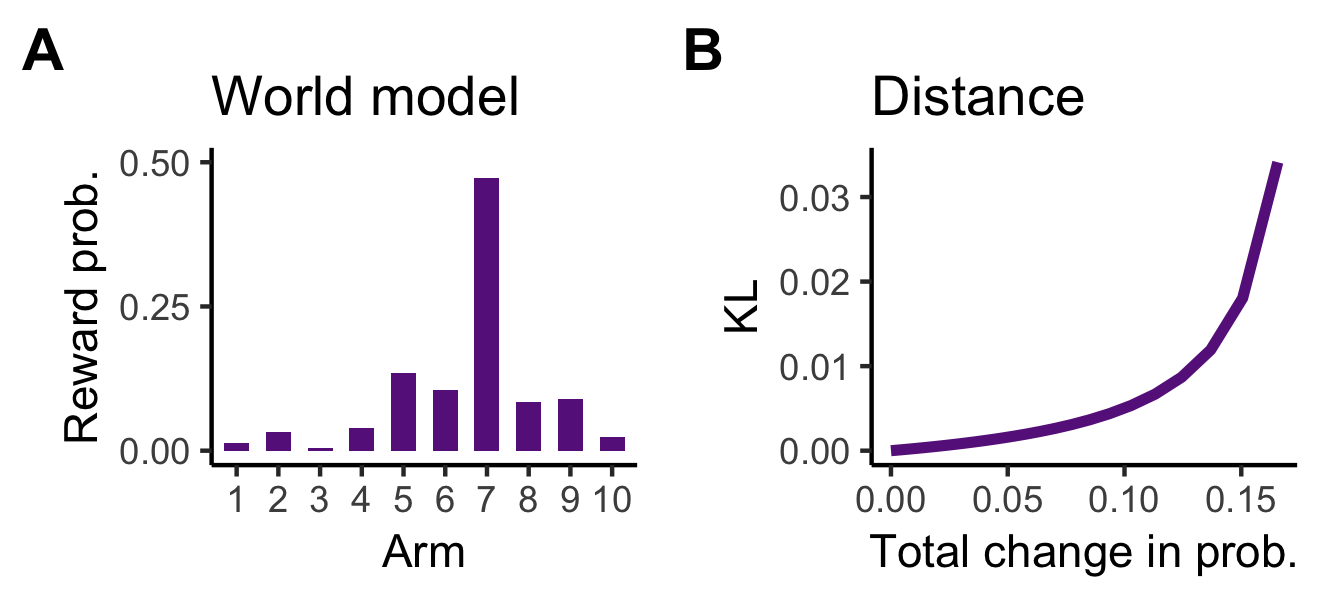
\includegraphics[width=.95\linewidth]{figures/subfig1.png} 
	\caption{\label{fig:supf1} A world model for bandits.
	\textbf{B}. Example of a single world model suitable for all bandit learning.
	\textbf{B} Changes in the KL divergence--our choice for the distance metric during bandit learning--compared to changes in world model, as by measured the total change in probability mass.}
\end{figure}

\begin{figure}
	[tbhp] \centering 
	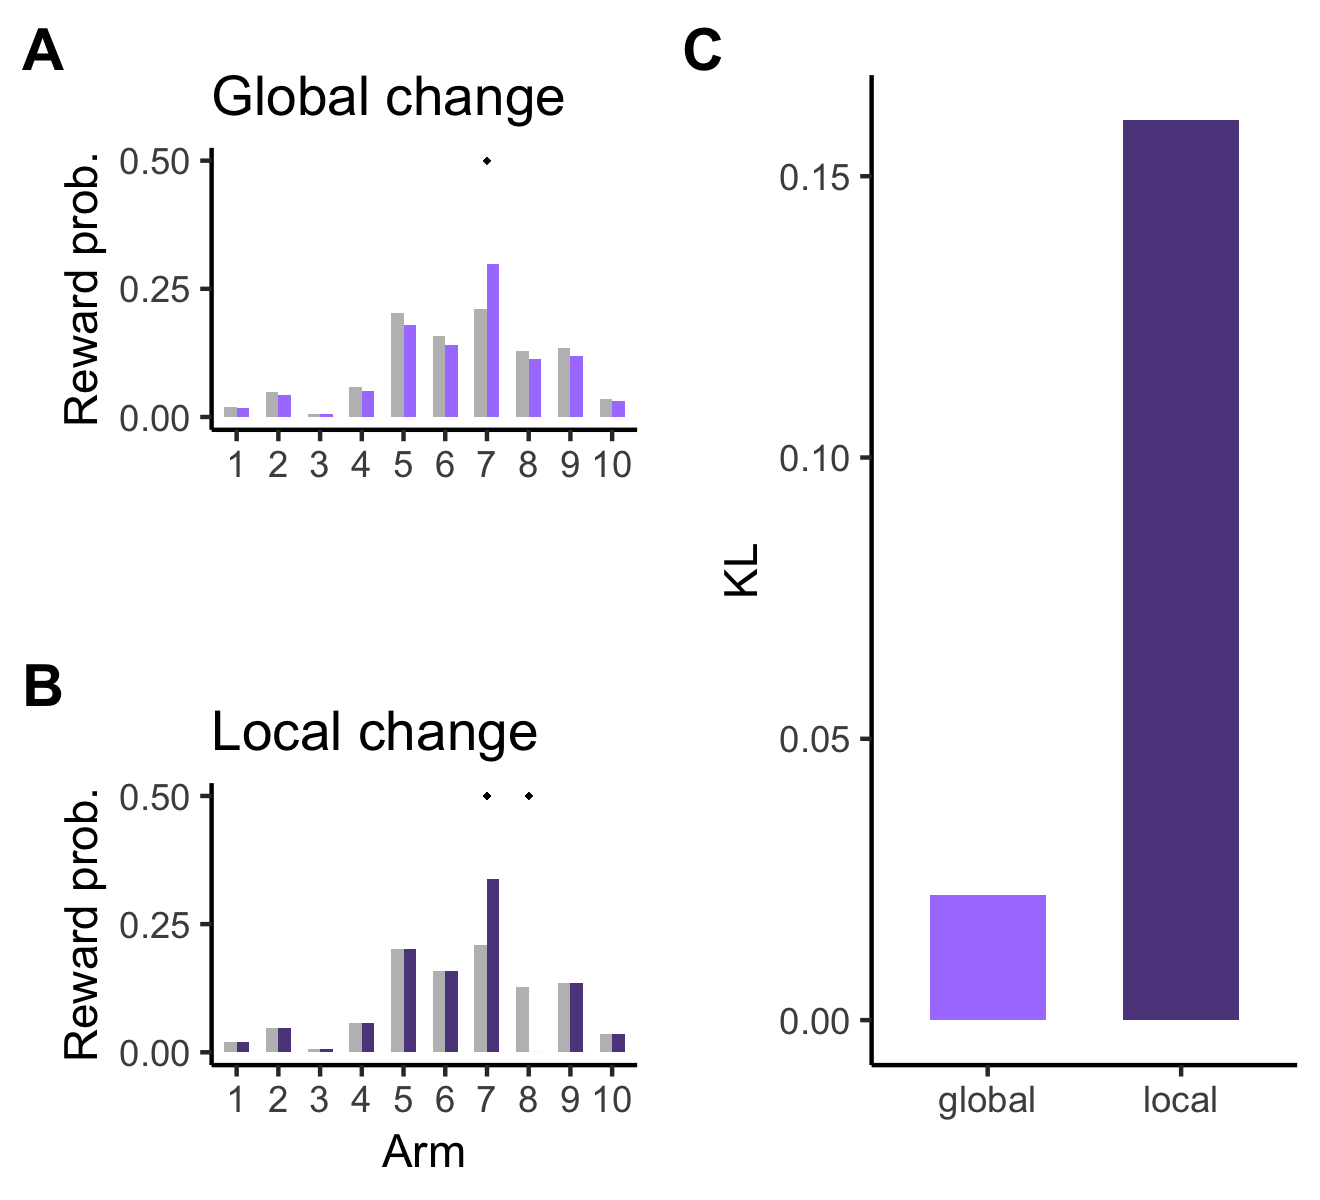
\includegraphics[width=.95\linewidth]{figures/subfig2.png} 
	\caption{\label{fig:supf2} An example of observation specificity during bandit learning. 
	\textbf{A}. A initial (grey) and learned (distribution), where the hypothetical observation $s$ increases the probability of arm 7 by about 0.1, and the expense of all the other probabilities.
	\textbf{B}. Same as A except that the decrease in probability comes only from arm 8.
	\textbf{C}. The KL divergence for local versus global learning.
	}
\end{figure}

\subsubsection*{Initializing $\pi_\pi$}
In these simulations we assume that at the start of learning an animal should have a uniform prior over the possible actions $A \in \mathbb{R}^K$. Thus $p(a_k) = 1/K$ for all $a_k \in A$. We transform this uniform prior into the appropriate units for our KL-based $E$ using Shannon entropy, $E_0 = \sum_K p(a_k)\ \text{log}\ p(a_k)$. 

In our simulations we use a tie breaking ``right next'' heuristic which keeps track of past breaks, and in a round robin fashion iterates rightward over the action space.

\subsubsection*{Reinforcement learning} Reinforcement learning in all agent models was done with using the TD(0) learning rule \cite{Sutton2018} (Eq. \ref{eq:TD}). Where $V(s)$ is the value for each state (arm), $\mathbf{R}_t$ is the \emph{return} for the current trial, and $\alpha$ is the learning rate $(0-1]$. See the \emph{Hyperparameter optimization} section for information on how $\alpha$ chosen for each agent and bandit.

\begin{equation}
	\label{eq:TD}
	V(s) = V(s) + \alpha (\mathbf{R}_t - V(s)
\end{equation}

The return $\mathbf{R}_t$ differed between agents. Our dual value agent, and both the variations of the e-greedy algorithm, used the reward from the environment $R_t$ as the return. This value was binary. The Bayesian reward agent used a combination of information value and reward $\mathbf{R}_t = R_t + \beta E_t$, with the weight $\beta$ tuned as described below. 

\subsubsection*{Hyperparameter optimization}
The hyperparameters for each agent were tuned independently for each bandit using a modified version of Hyperband \cite{Li2016a}. For a description of hyperparameters seen Table \ref{tab:agents}, and for the values themselves Table~\ref{table:hp}.

\begin{table}[]
\caption{Hyperparameters for individual bandits (\textbf{I}-\textbf{IV}).}
\label{tab:hp}
\begin{tabular}{|l|l|l|l|l|l|}
\hline
\textbf{Agent} & \textbf{Parameter} & \textbf{I} & \textbf{II} & \textbf{III} & \textbf{IV} \\ \hline
Dual value & $\eta$ & 0.053 & 0.017 & 0.003 & 5.8e-09 \\ \hline
Dual value & $\alpha$ & 0.34 & 0.17 & 0.15 & 0.0011 \\ \hline
E-greedy & $\epsilon$ & 0.14 & 0.039 & 0.12 & 0.41 \\ \hline
E-greedy & $\alpha$ & 0.087 & 0.086 & 0.14 & 0.00048 \\ \hline
Annealed e-greedy & $\tau_E$ & 0.061 & 0.084 & 0.0078 & 0.072 \\ \hline
Annealed e-greedy & $\epsilon$ & 0.45 & 0.98 & 0.85 & 0.51 \\ \hline
Annealed e-greedy & $\alpha$ & 0.14 & 0.19 & 0.173 & 0.00027 \\ \hline
Bayesian & $\beta$ & 0.066 & 0.13 & 0.13 & 2.14 \\ \hline
Bayesian & $\alpha$ & 0.066 & 0.03 & 0.17 & 0.13 \\ \hline
Bayesian & $\gamma$ & 0.13 & 0.98 & 0.081 & 5.045 \\ \hline
\end{tabular}
\end{table}

\subsubsection*{Exploration and value dynamics}. 
While agents earned nearly equivalent total reward in Bandit I (Fig~\ref{fig:f3}, \textit{top row}), their exploration strategies were quite distinct. In Supp. Fig~\ref{fig:supf3}\textbf{B}-\textbf{D}) we compare three prototypical examples of exploration, for each major class of agent: ours, Bayesian, and E-greedy for Bandit \textit{I}. In Supp. Fig~\ref{fig:supf3}\textbf{A}) we include an example of value learning value learning in our agent.

\begin{figure}
	[tbhp] \centering 
	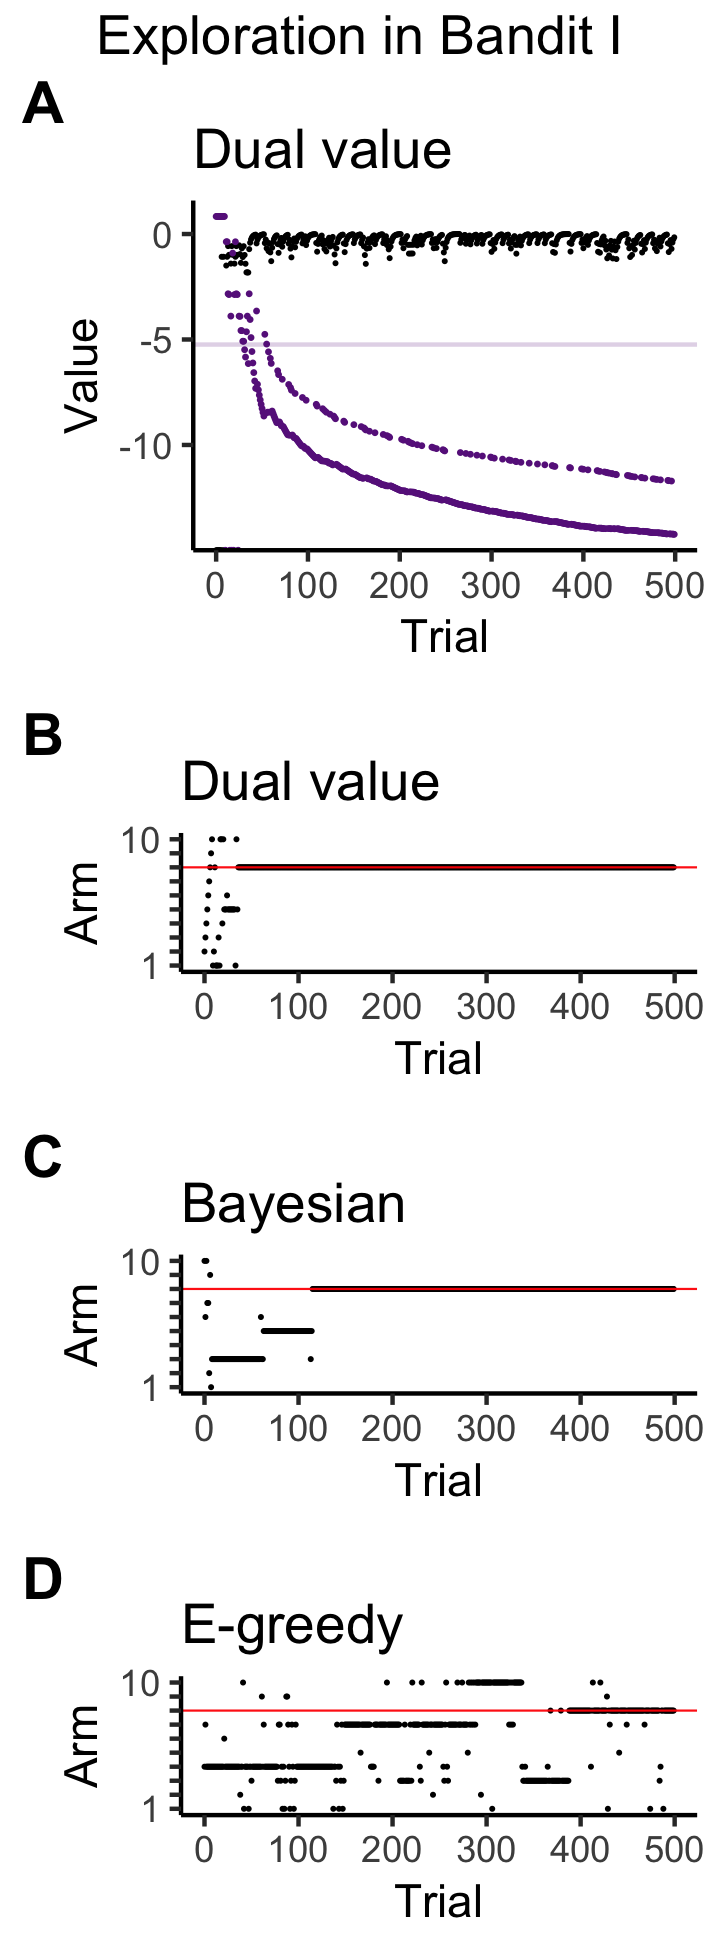
\includegraphics[width=.5\linewidth]{figures/subfig3.png} 
	\caption{\label{fig:supf3} Exploration and value dynamics.
	\textbf{A}. An example of our dual value learning algorithm during 500 trials on Bandit. The light purple line represents the boredom threshold $\eta$ (Eq.~\ref{eq:pipi}).
	\textbf{B.} An example of exploration dynamics (i.e arm selection) on Bandit. Note how the search is structured, and initially sequential.  
	\textbf{C-D.} Exploration dynamics for two other agents. \textbf{C.} The Bayesian agent, which like our algorithm uses active sampling, and values information. Note how this shows a mixture of structures and repeated choices, mixed with seemingly random behavior. \textbf{D.} The E-greedy agent, which uses purely random sampling. Note how here the agent is either greedy, repeating the same arm, or seemingly random.}
\end{figure}


\end{document}